\documentclass[a4paper,10pt]{article}
\usepackage[utf8]{inputenc}
\usepackage{fullpage}
\usepackage{cite}
\usepackage{graphicx}
\usepackage{wrapfig}
\usepackage{url}
\DeclareGraphicsExtensions{.pdf,.eps,.svg,.pgm}
    % EXTREMELY COMMON LaTeX PACKAGES TO INCLUDE:
    \usepackage{amsmath,amsthm, amsfonts,amssymb} % For AMS Beautification
    \usepackage{setspace} % For Single & Double Spacing Commands
    \usepackage[linktocpage,bookmarksopen,bookmarksnumbered,% For PDF navigation
		pdftitle={Group 2: Sotiriou et. al.},%   and URL hyperlinks
		pdfauthor={Department of Electronic and Computing Systems},%
		pdfsubject={UC },%
		pdfkeywords={UC}]{hyperref}
           \usepackage{caption3} % load caption package kernel first
    \DeclareCaptionOption{parskip}[]{} % disable "parskip" caption option
    \usepackage[small]{caption}
\usepackage{amsmath}
\usepackage{amsfonts}
\usepackage{amsthm}
%opening
\title{Assessing Histological Grades of Primary Breast Cancer Using Gene Signatures}
\author{Priyanka Arora, Lee Carraher,Ben Landis, Li Jing, Samuel Schmidt}
\begin{document}

\maketitle

\begin{abstract}
This paper is a re-Analysis of the Sotiriou et. al. paper on using tumor 
histological grade expressed gene signatures for breast cancer 
prognosis\cite{Sotiriou}. The principle assumptions of this process are that
the classification of histological grade and tumor progression has a strong 
correlation with the length of survival time. Furthermore, we suggest grade 2
tumors are misclassified grade 1 or grade 3 tumors. The result of developing 
better gene signatures for classifying tumor grades can further
assist in diagnosis and treatment options for breast cancer patients.


\end{abstract}

\section{Background}
\section{Purpose and Hypothesis}
\section{Methods and Materials}
\subsection{Data Acquisition and Sampling}


Five gene expression datasets were used in this study which were obtained by
 microarray analysis (using  Affymetrix U133A Genechips) of tumor samples
 from 661 patients with primary breast cancer. \\
They are enumerated below:\\
\begin{itemize}
 \item The training set KJX64.
 \item The validation set KJ125.
 \item The National Cancer Institute (NCI) dataset from Sotiriou et al. \cite{Sotiriou1}
 \item The Stanford/Norway (STNO) dataset from Sorlie et al. \cite{Sorlie1}
 \item The Nederlands Kanker Instituut (NKI) 2 dataset from Van de Vijver et al. \cite{Vijver1}
\end{itemize}

Histologic tumor grade in these datasets was based on the Elston – 
Ellis grading system \cite{Elston1} and the standardized mean difference of Hedges 
and Olkin \cite{Hedges1} was used to rank genes by their differential expression. The probe 
sets of the Affymetrix U133A Genechips were mapped to other microarray platforms
 by matching the Unigene identifiers (version 180), following the technique mentioned in Praz et al. \cite{Cleanex}
For gene expression analysis, RNA was isolated by utilization of TRIzol, which 
is a monophasic solution of phenol and guanidinium isothiocyanate, used for 
solubilizing biological material and denaturation of proteins. Agilent Bioanalyzer 
was used for optimization and quality control of the RNA obtained from all those
 tumor samples and only the ones with good quality of RNA were acknowledged for further examination. 
For the purpose of our analysis, while selecting the grade-associated genes, 
we only considered the ER-positive tumors and excluded the ones with ER-negative
 and NA status on account of the relationship between the ER status and histologic 
grade. As mentioned in the Sotiriou et al. paper \cite{Sotiriou}, majority of the ER-negative tumors
 are grouped as either intermediate (Grade 2) or high (Grade 3) histologic grade, 
assuming that we had utilized all histologic grade 1 and 3 tumors despite their ER 
status during our analysis, we might have ended up choosing ER-identified genes
 that were falsely connected with grade.


\subsection{Differential Expression Modeling Methods}
Our method of assessing histological grade of primary breast cancer consists of three phases. The first phase is
a semi-supervised ranking of genes and grade 1 and grade 3 tumors based on maximum differential
expression. The second phase consists of selecting a set of genes that are up-regulated with 
grade 3 tumors and down regulated in grade 3. In the third phase, we generated two groups of tumor samples.
Classification of the grade 2 tumors is then performed using these groups as models. Below we expand upon
our process in detail.\\
The gene signature identification process consisted of assessing the Sotiriou breast cancer data set with Genomics Portals (genomicsportals.org).
Genomics portals performs differential analysis on genes and samples using the CLEAN algorithm\cite{CLEAN}. CLEAN co-clusters
the genes and sample grades hierarchically, using data from the dataset and a database of known gene functional groups. Highly differentially
expressed genes were identified with a p-value of .001, and fold change over expression level of 2. The results of this analysis
were inspected in genomics portal's Treeview navigator\cite{Treeview}, and the visually most cohesive up-regulated set of genes
corresponding to grade 3 tumors was selected as our gene signature\ref{grade13diff}. Inspection with Treeview failed to suggested a 
visually significant cluster of down-regulated genes for grade 3 tumors, therefore only up-regulated ones were included in our model. 
We acquired a set of 49 differentially expressed up-regulated grade 3 tumor genes from this analysis.\\
\begin{figure}
\centering
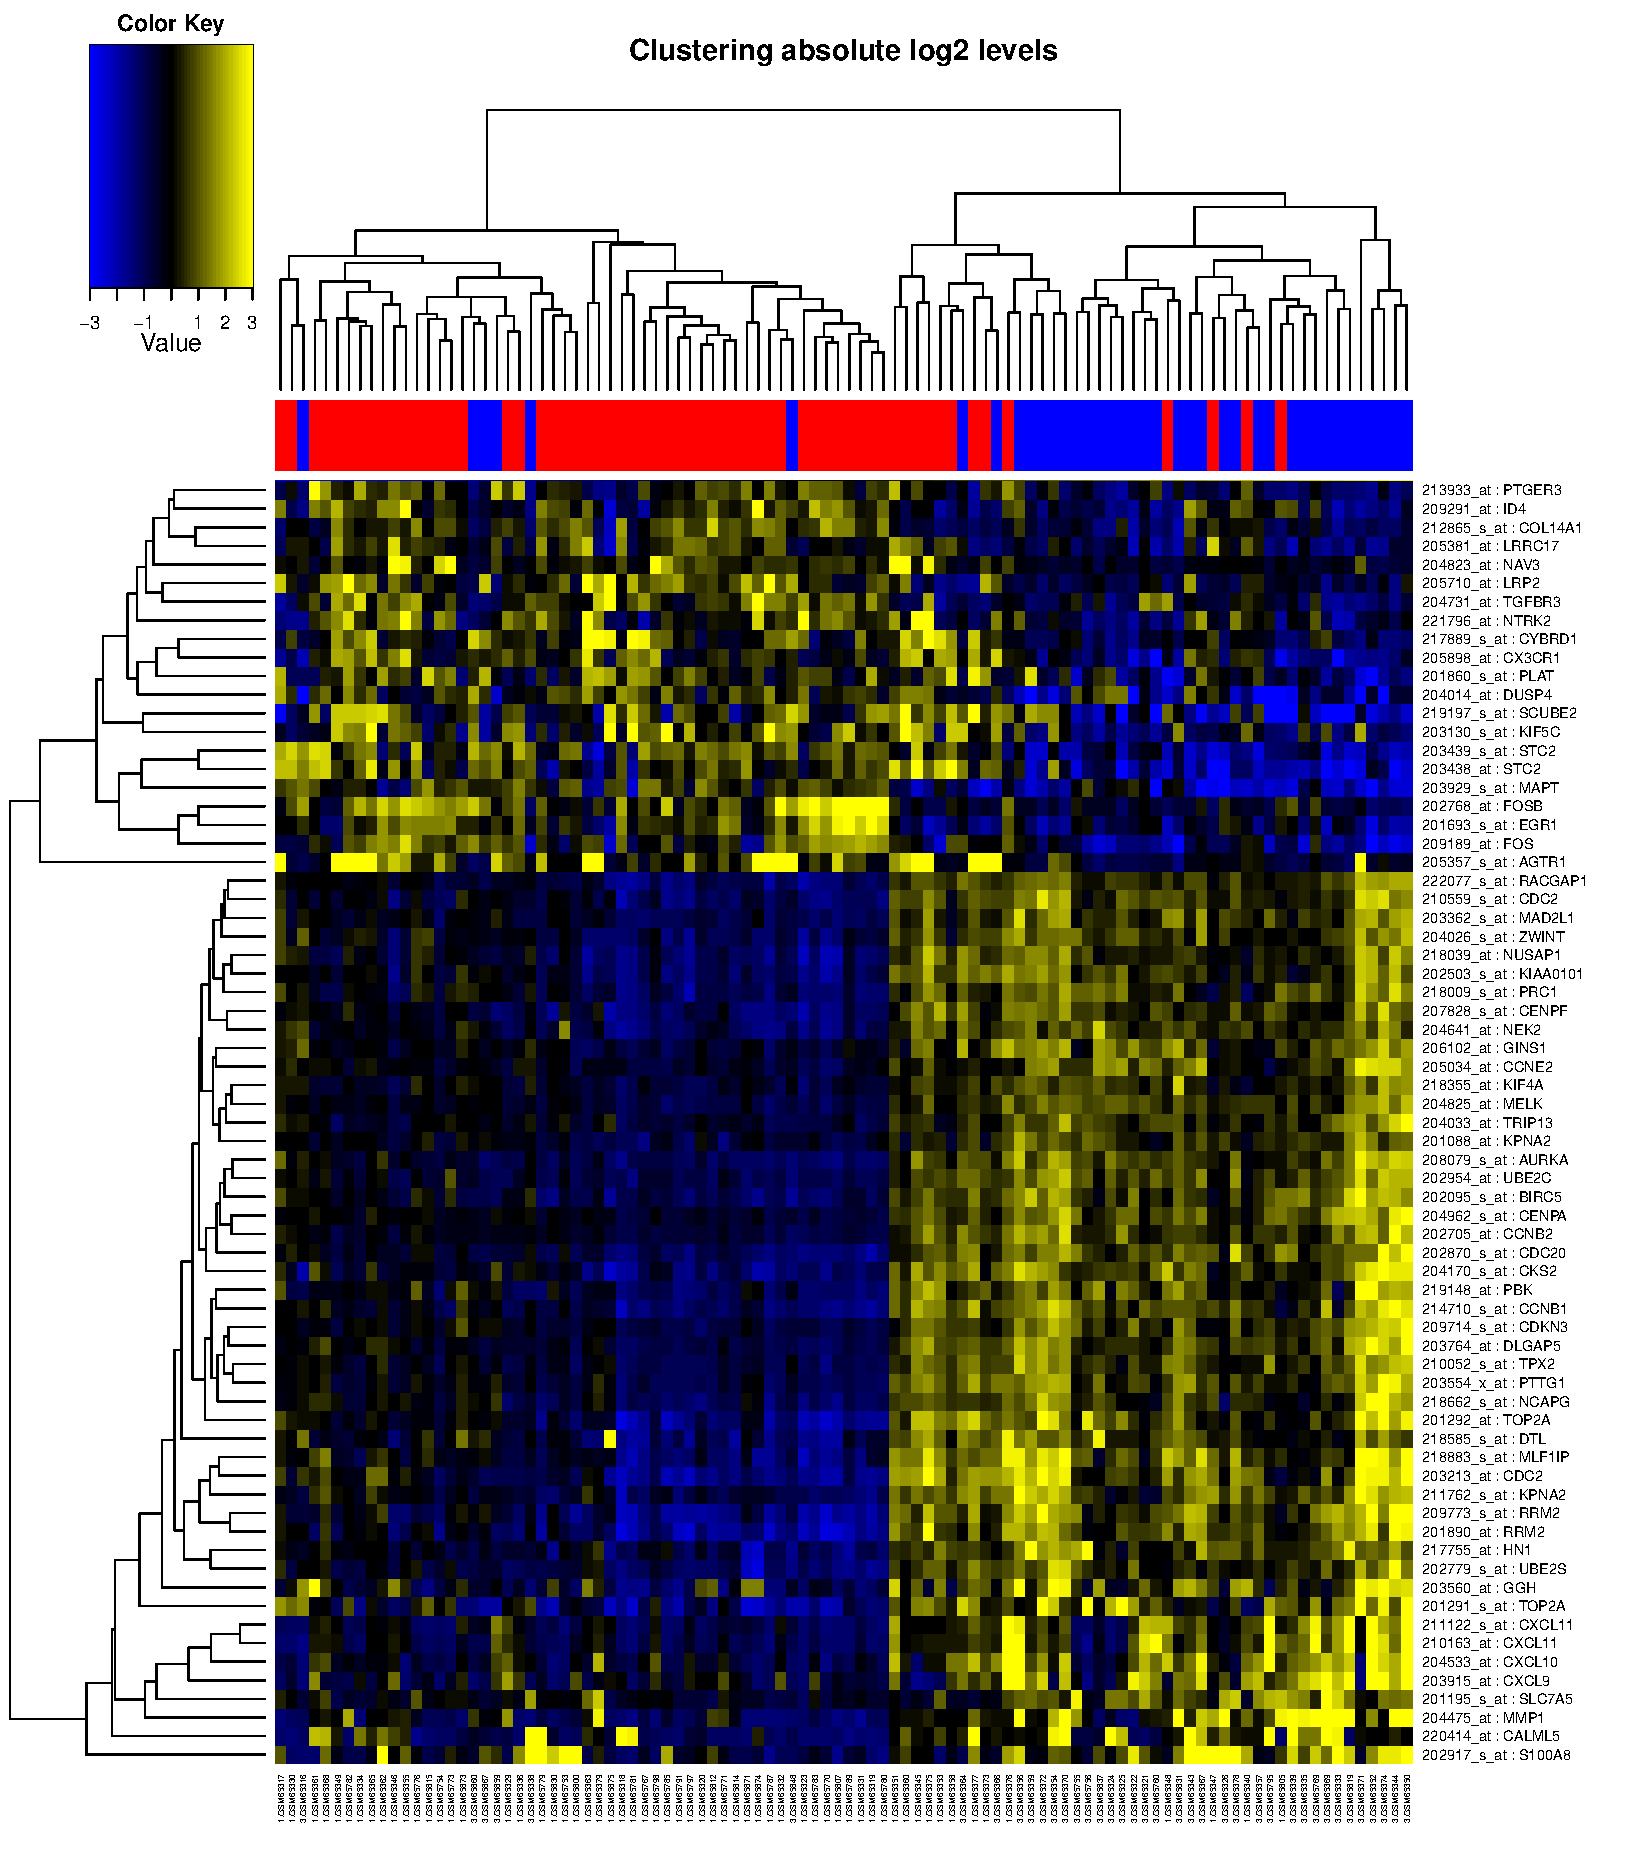
\includegraphics[scale=0.30]{docs/grade1and3differentiallyexpressed}
\caption{Grade 1 and Grade 3 Differentially Expressed}\label{grade13diff}
\end{figure}
Using the selected set of 49 genes as a signature we supposed a $|$gene signature$|-$dimensional subspace to build our model.
Withing the subspace, we used the clinically provided grade labels to generate centroids for the two , 1 and 3 - grade, groups following
the expression (Figure \ref{centroid}) . Noise suppression refinement was performed by removing samples that deviated from the group cluster
centers by more than 2 standard deviations of the cluster's mean variance.\\
\begin{figure}
$$
Centroid(Grade_X)= \left[              \underset{x\in X}     \sum{  { {x_1}    \over {| X |} } }   ,   
 \underset{x\in X}     \sum{  { {x_2}    \over {| X |} } },
\ldots ,
 \underset{x\in X}     \sum{  { {x_{| gene signature |}}    \over {| X |} } }                 \right] 
$$
\caption{Grade Gene Expression Centroid Generation}\label{centroid}
\end{figure}
For visual assessment of our analysis, we queried the grade 2 tumors against the grade 1 and 3 differentially expressed genes. The resulting chart
shows a distinct clustering between the grade 1-like and grade 3-like tumors that follow approximately 
the grade 3 and grade 1 distributions. Assuming the dataset comprises the actual distribution 
of grade 1 to grade 3 tumors, approximately 55:64 for grade 1 and grade 3 respectively (figure \ref{grade2up}) we reassert our hypothesis
of the lack of a grade 2 class distinction.
\begin{figure}
\centering
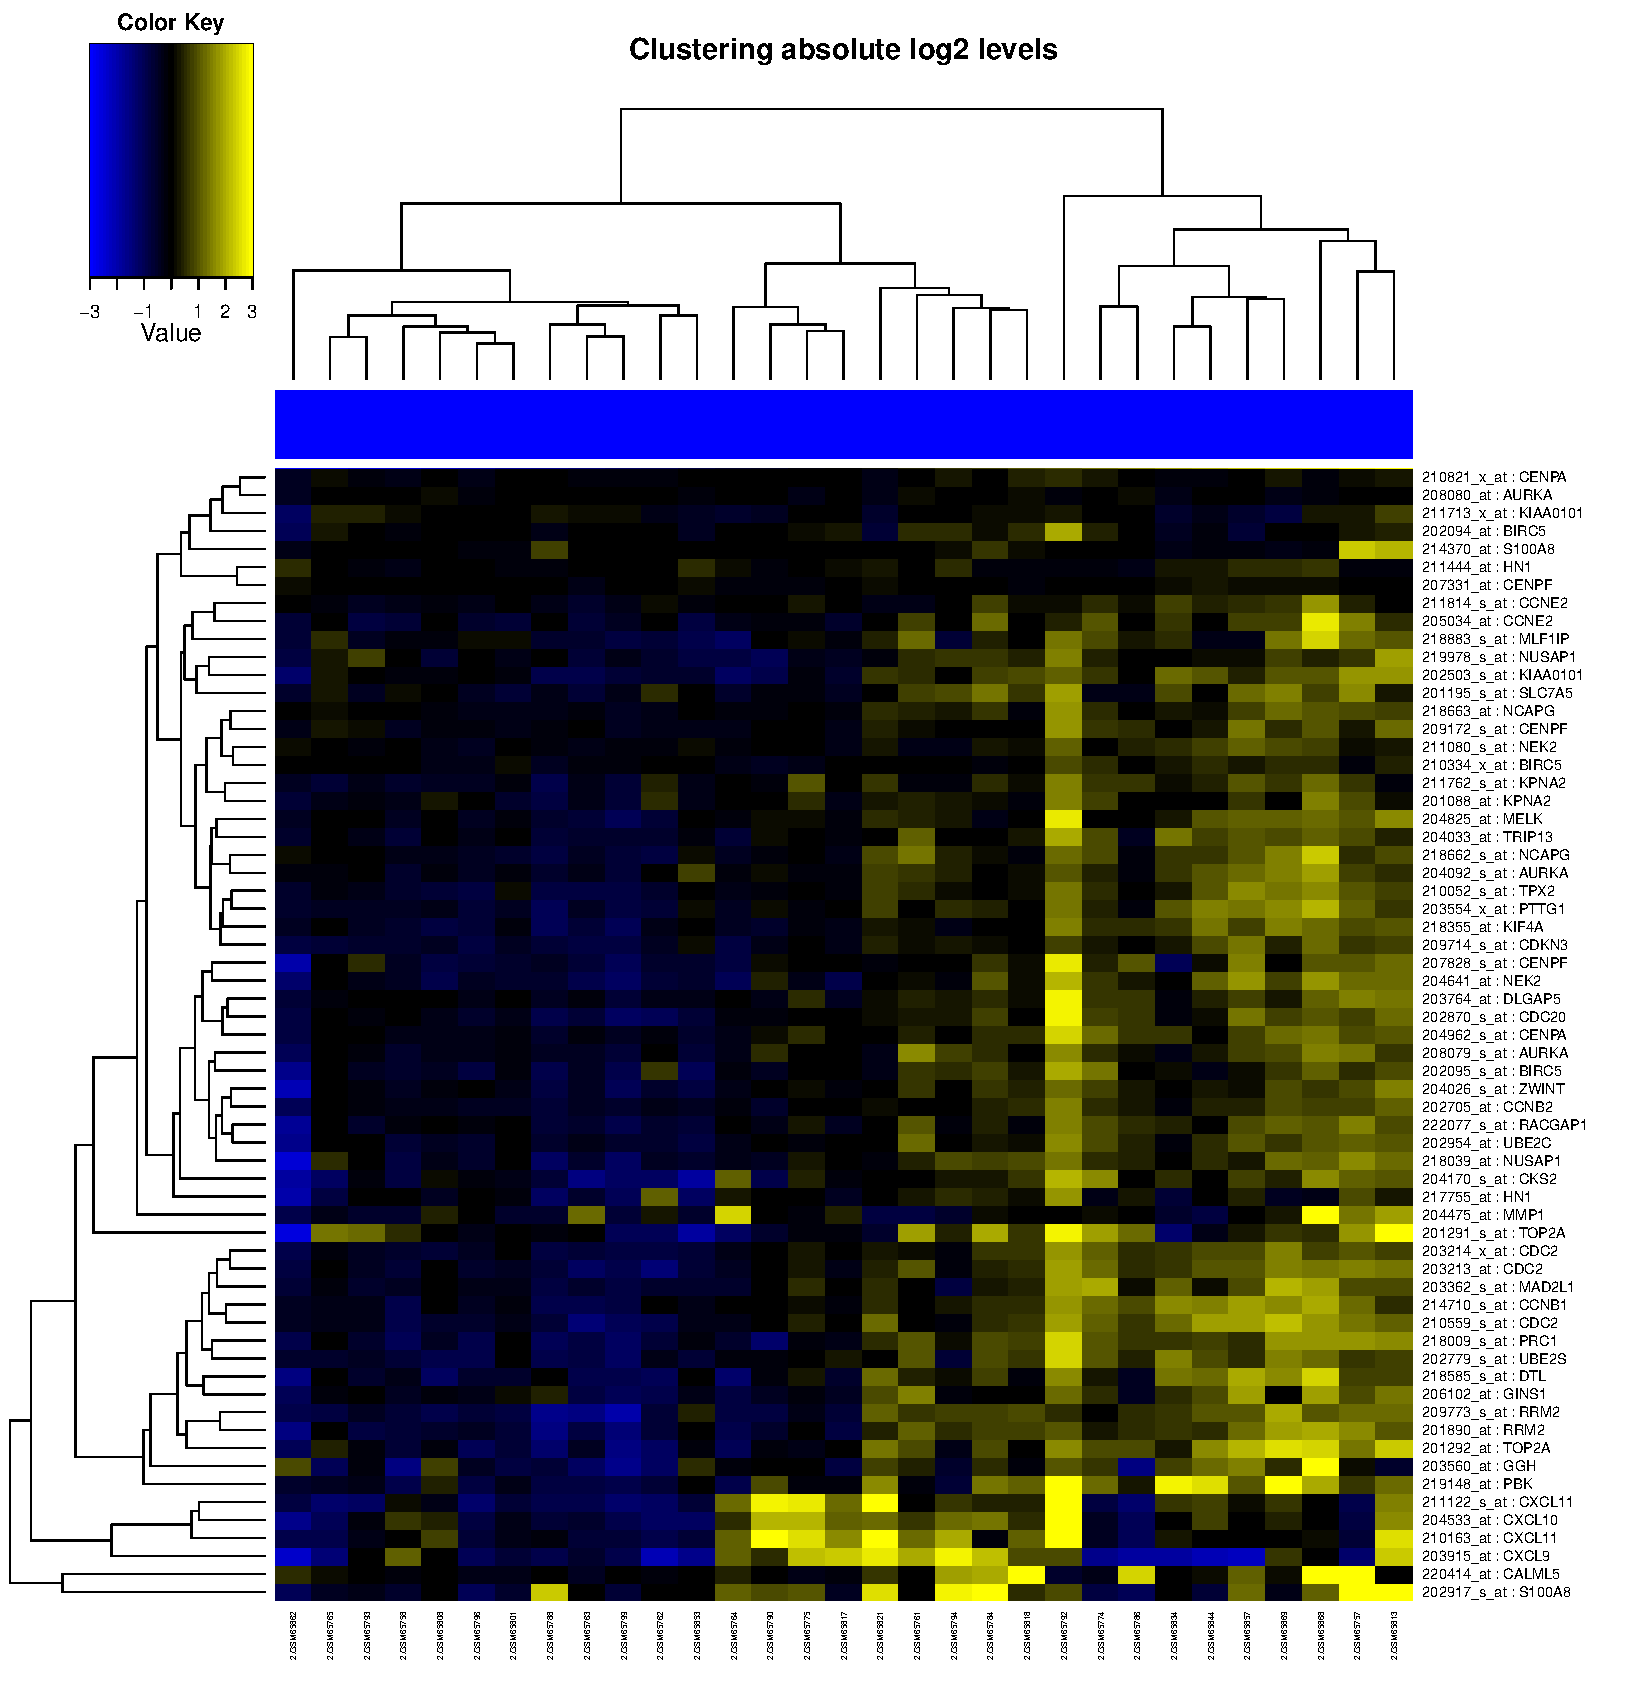
\includegraphics[scale=0.30]{docs/grade2onupregulated3}
\caption{Grade 2 Differentially Expressed Genes from Grade 1 and Grade 3}\label{grade2up}
\end{figure}
\begin{figure}
 $$
Grade(X) = \underset{C \in Centroids} {\mathrm{argmin}} ~ \left( \sqrt{\sum_{g\in genelist}{ (X_{g} - C_{g})^2}}\right)
$$
\caption{Nearest Centroid Classification}\label{classify}
\end{figure}
Classification of grade 2 tumors was then computed by nearest centroid under the euclidean norm following the method in figure \ref{classify}.
The new classifications were then used to recompute the KM-Survival analysis on tumor grades 2A (or grade 1-like) and 2b (or grade 3-like).



\subsection{Other Unsupervised Learning Methods}
In addition to the use of genomics portals to identify differentially expressed genes, two common unsupervised machine learning techniques were
used to classify histological grades based on genetic expression. The first method used was the K-Means method. We will forgo an exhaustive explanation
of K-Means here as it is a long known method with many descriptions and analysis available online. K-Means is an unsupervised clustering method
that attempts to minimize the inter-cluster distance on a set of N points and K cluster assignments. The method is greedy and iterative, with few guarantees
on optimality, however combined with random starts, the overall performance of K-Means is actually quite good for spherical clusters\cite{kmeans}. 
For our testing, following our aforementioned hypothesis of the existence of only two genetically identifiable tumor grades (low and high), we performed
100 tests using K-Means on 50:50 training:test data comprising grade 1 and grade 3 tumors. The reclassification accuracy results are given in (\ref{KMResults}).
\begin{itemize}\label{KMResults}
\item Mean 0.8382
\item Mode 0.84
\item Min 0.58
\item Max 0.94
\item Var 0.00315
\end{itemize}
From the results it is clear there is significant error in the upper and lower bounds for accuracy. This though partially due to the K-Means algorithm
itself, may have resulted from a badly conditioned training and test dataset split. As 50\% grade 1 and 50\% grade 3 would suggest the optimal split,
we assert that the actual min accuracy performance is slightly lower than the real performance of K-Means, while the max is no better than could
ideally be achieved from random 50:50 splitting.\\
The second unsupervised method, Projection to Latent Structures Regression (or Partial Least Squares Regression, \emph{PLSR})\cite{Wold1} proved to 
be slightly less accurate in its ability to correctly classify data. Despite its accuracy performance shortcomings, it did however
perform well in its ability to identify highly differentially expressed genes.

%Computed centroids for grades 1 and 3 based on the 49 up-regulated genes identified with genomic portals.\cite{Treeview},\cite{CLEAN}

%Used those centroids to reclassify grade 2 tumors using Nearest Centroid based on Euclidean distance.

%* Projection to Latent Space Regression (PLSR) on 49, 7231, and 11467 genes.
%on 50:50 train, test data. 
%* Identifies 6 genes: 2 calcium related proteins and 4 chemokines
%* Unsupervised k-means was
%  applied, with similarly poor classification     performance.
%* Performed similar analysis with PAM50 
%* Qualitatively the heatmap results were worse, as PAM50 is for subtype classification.
%* Interestingly, nearest centroid assignment was almost identical.
%Up-regulated genes from grade 3 and 1 differential expression applied to grade 2 tumors (Figure \ref{grade2up})

\section{Results and Discussion}
\section{Conclusion}
90\% of the time it works all the time!
\bibliography{refs}
\bibliographystyle{ieeetr} \markright{ }


\end{document}
